\documentclass{article}
\textheight = 25cm
% largo texto impreso
\textwidth = 18cm % ancho texto impreso
\topmargin = -2cm % margen superior 3-2=1cm
\oddsidemargin = -2cm
% margen izquierdo 4.5-2=2.5cm
% Sangría=0mm
\parindent = 0mm
\usepackage{graphicx}
\usepackage[T1]{fontenc} % fuentes adecuadas para salida % acentos,etc., desde el teclado
\usepackage{amsmath,amssymb,amsfonts,latexsym}
\usepackage{graphicx}
\usepackage[shortlabels]{enumitem}
\usepackage{esvect}
\usepackage{mathtools}
\usepackage{graphicx}
\usepackage[a4paper,margin=2cm,noheadfoot]{geometry}
\usepackage{float}
\usepackage{xspace,color}
\usepackage{url}
\usepackage{listings}



\lstset{commentstyle=\color{red},keywordstyle=\color{black},
showstringspaces=false}
\lstnewenvironment{rc}[1][]{\lstset{language=R}}{}
\newcommand{\ri}[1]{\lstinline{#1}}  %% Short for 'R inline'
\lstset{language=R} 


\begin{document}
\parbox{3.3cm}{
\includegraphics[width=3cm]{Images/usblogo.eps}}\parbox{8cm}{Universidad
   Sim\'on Bol\'ivar\\
   Departamento de C\'omputo Cientifico y Estadistica
   \hspace{1cm}CO5316 An\'alisis de Datos\\
   Informe an\'alisis exploratorio}\parbox{17cm}{ \hspace{1cm}Alimi Garmendia 14-10392\\
  \hspace*{1cm}Rafael Garcia Sanchez 14-11180 \\
  \hspace*{1cm}Orlando Chaparro 12-11499 \\
   \hspace*{1cm}Enero 2020}
   \vspace{1cm}

    En este informe nos enfocaremos en los alumnos pertenecientes a los grupos \'etnicos A y E, por lo cual comenzaremos an\'alizando
    su representaci\'on en el sal\'on y compararemos su desempe\~no en las materias.
    

    \begin{figure}[h]
        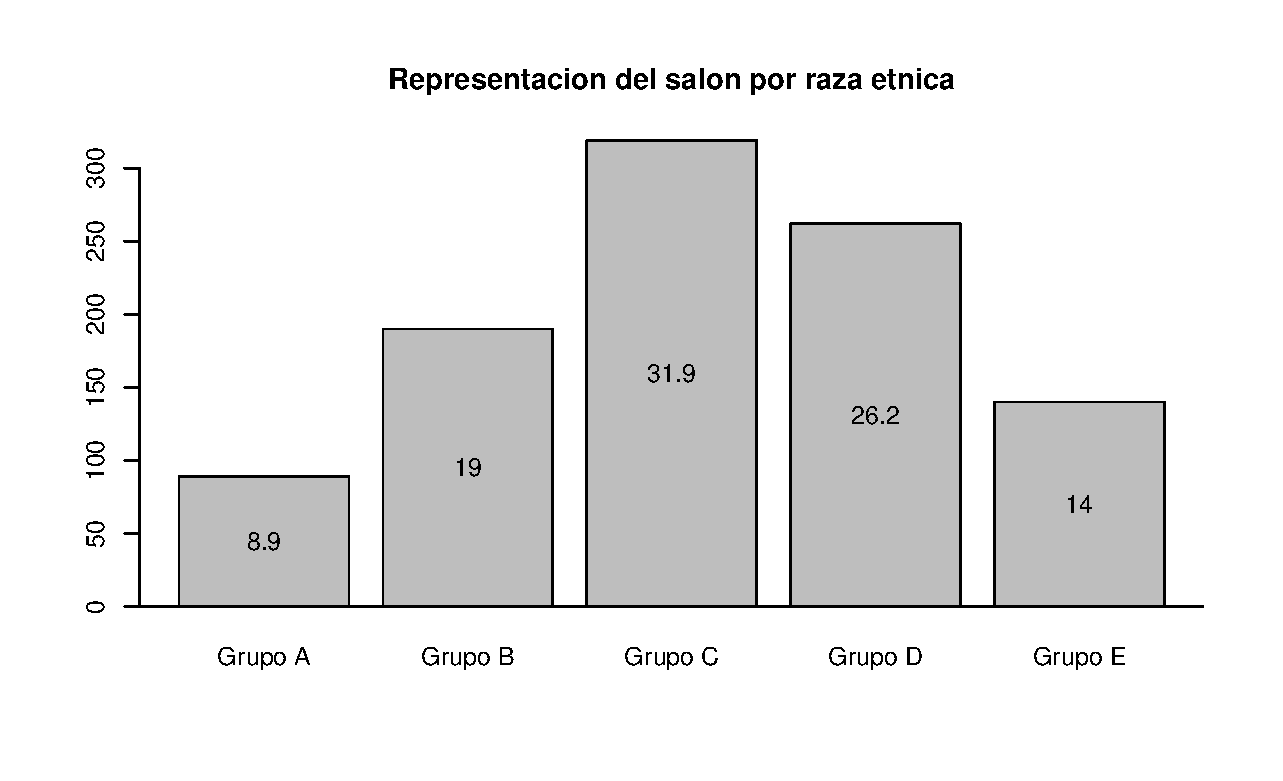
\includegraphics[scale = 0.8]{Output/Plots/1_Representaciondelsalonporrazaetnica.eps}
        \caption{Representaci\'on del sal\'on por raza \'etnica}
        \label{fig:minipage1}
    \end{figure}

    Los grupos A y E, como podemos ver en la figura 1, son los dos grupos con menos representaci\'on en el sal\'on, por lo
    que analizaremos su desempe\~no respecto a los dem\'as grupos \'etnicos.

    \vspace*{-4mm}
    \begin{figure}[H]
        \noindent\makebox[\textwidth]{
        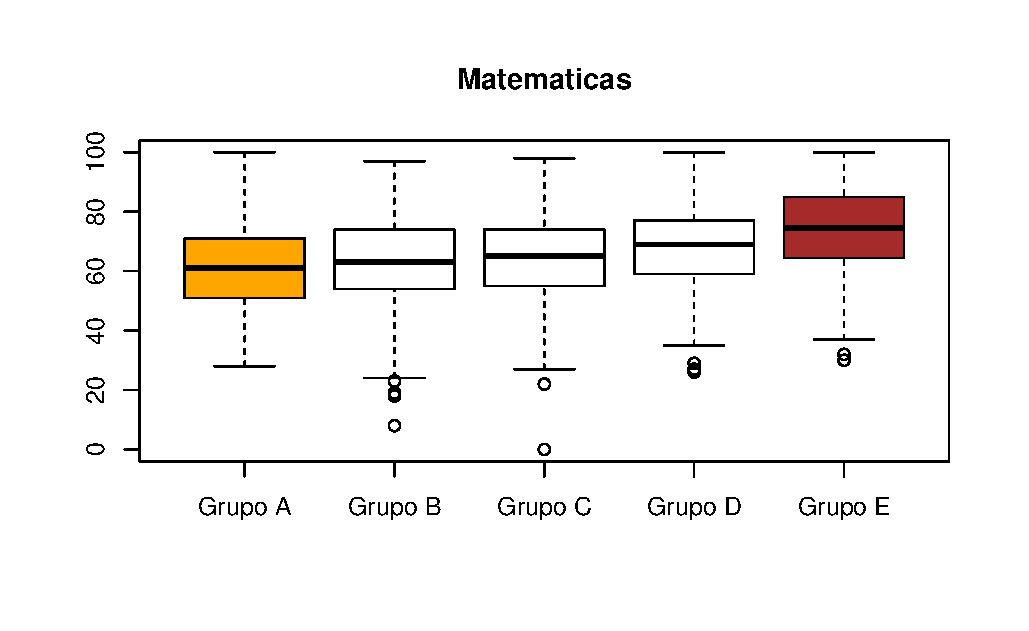
\includegraphics[scale = 0.8]{Output/Plots/2Mathgrupos.eps}}
        \vspace*{-20mm}
        \caption{Resultados en Matem\'aticas}
        \label{fig:minipage1}
    \end{figure}
    \vspace*{-20mm}

    \begin{figure}[H]
        \noindent\makebox[\textwidth]{
        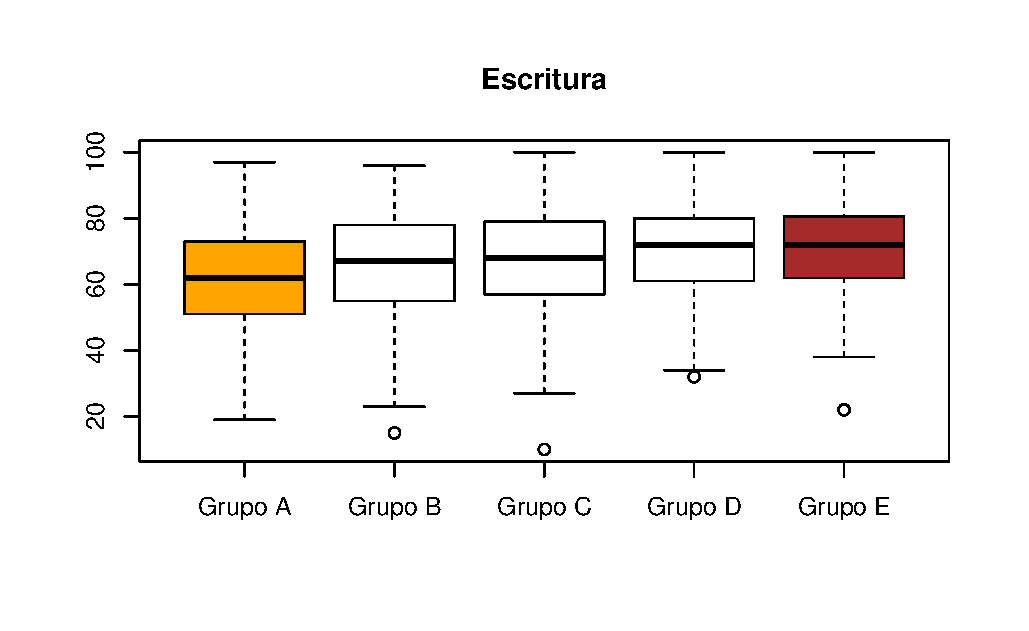
\includegraphics[scale = 0.8]{Output/Plots/Writtinggrupos.eps}}
        \vspace*{-20mm}
        \caption{Resultados en Escritura}
        \label{fig:minipage1}
    \end{figure}

    \vspace*{-9mm}
    \begin{figure}[H]
        \noindent\makebox[\textwidth]{
        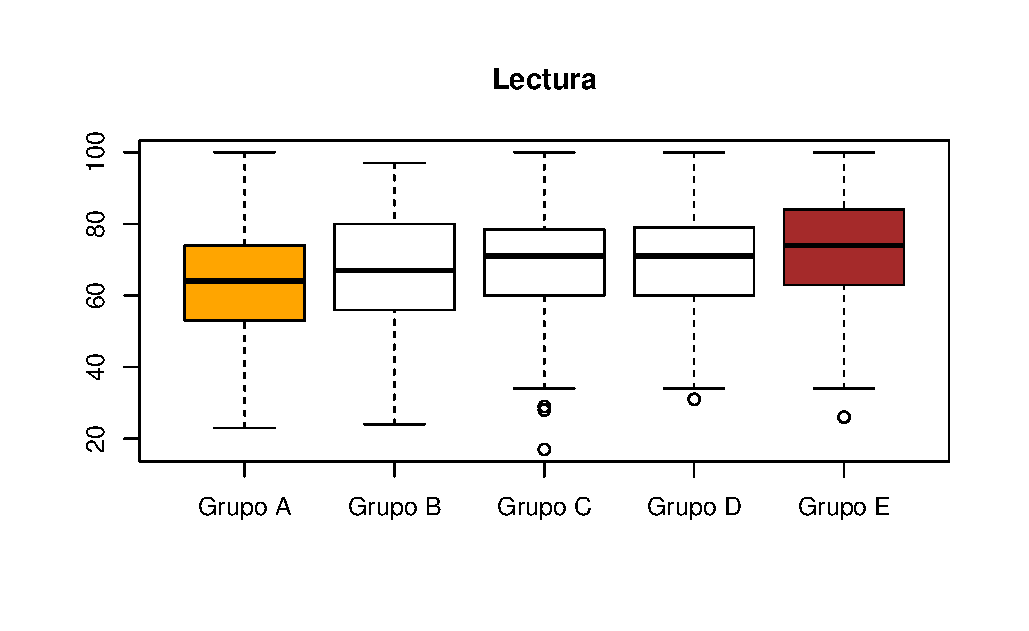
\includegraphics[scale = 0.8]{Output/Plots/Readinggrupos.eps}}
        \vspace*{-20mm}
        \caption{Resultados Lectura}
        \label{fig:minipage1}
    \end{figure}
     
    Es muy resaltante las diferencias entre ambos grupos, mientras que A en promedio fue el grupo menos favorecido en las
    tres pruebas, el grupo E pareciera tener mucho mejores resultados. Ahora nos concentraremos en analizar si las variables
    provistas dan alguna pista sobre la disparidad en los puntajes obtenidos.

    \begin{figure}[H]
        \begin{minipage}[b]{0.45\linewidth}
            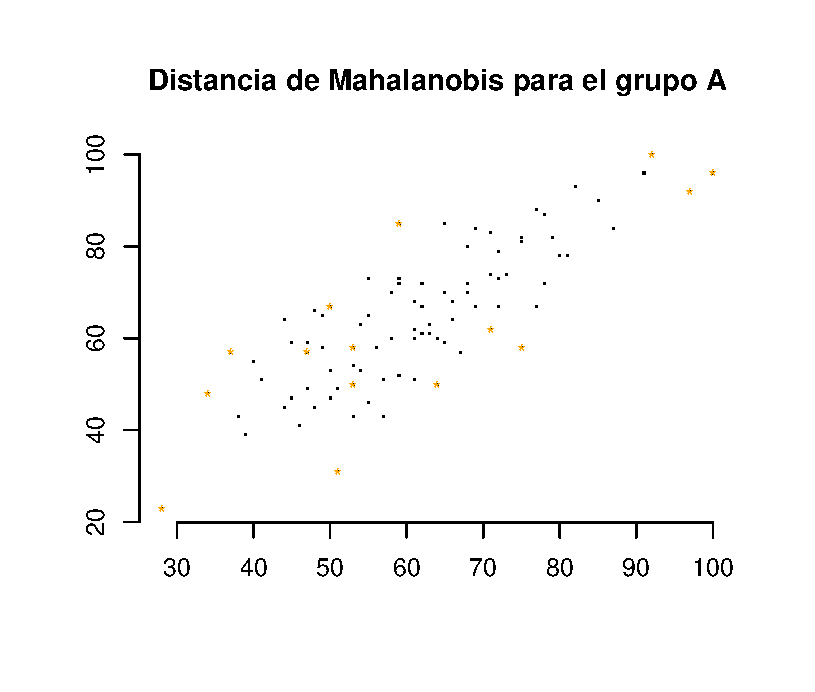
\includegraphics[scale = 0.4]{Output/Plots/MahalanobisA1.eps}
            \vspace*{-6mm}
            \caption{Representaci\'on de la distancia de Mahalanobis grupo A}
            \label{fig:minipage1}
        \end{minipage}
        \hspace{0.2cm}
        \begin{minipage}[b]{0.45\linewidth}
            \includegraphics[scale = 0.4]{Output/Plots/MahalanobisA2.eps}
            \vspace*{-6mm}
            \caption{Representaci\'on de la distancia de Mahalanobis grupo A}
            \label{fig:minipage2}
        \end{minipage}
    \end{figure}
    \begin{figure}[H]
        \begin{minipage}[b]{0.45\linewidth}
            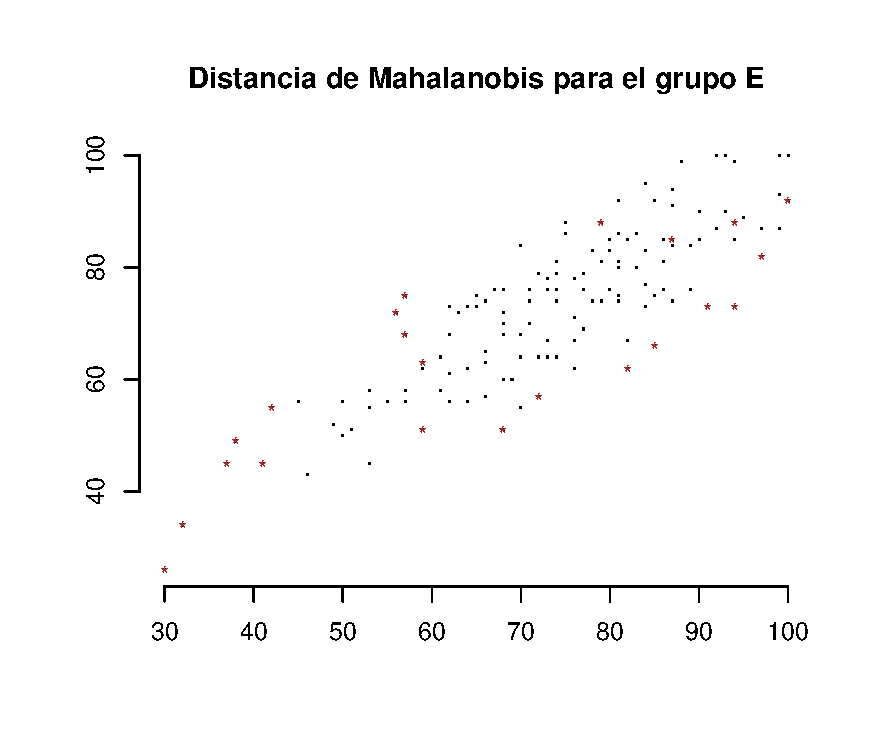
\includegraphics[scale = 0.4]{Output/Plots/MahalanobisE1.eps}
            \vspace*{-6mm}
            \caption{Representaci\'on de la distancia de Mahalanobis grupo E}
            \label{fig:minipage1}
        \end{minipage}
        \hspace{0.2cm}
        \begin{minipage}[b]{0.45\linewidth}
            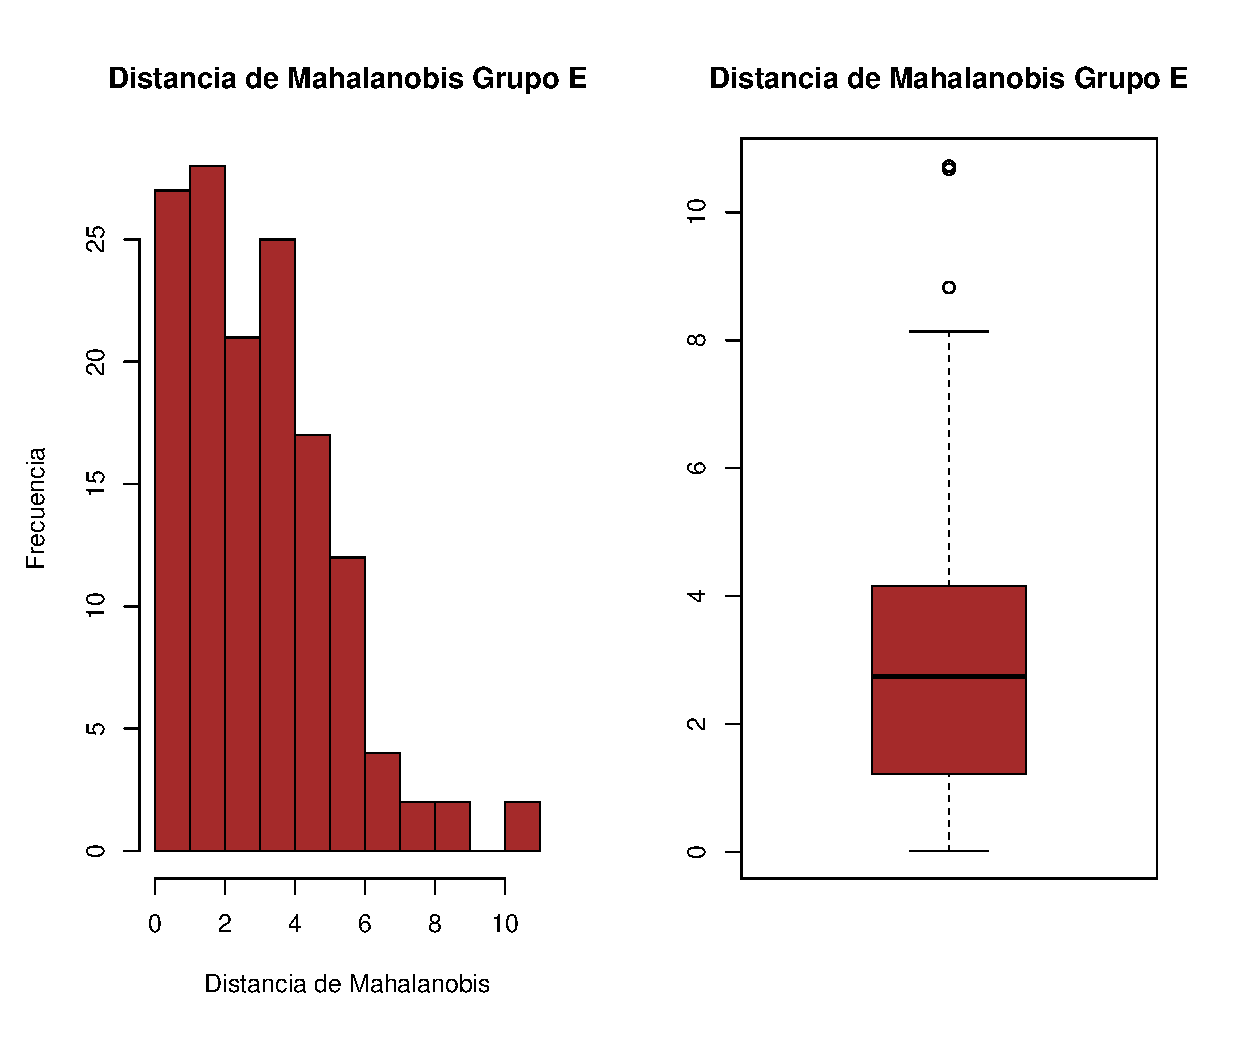
\includegraphics[scale = 0.4]{Output/Plots/MahalanobisE2.eps}
            \vspace*{-6mm}
            \caption{Representaci\'on de la distancia de Mahalanobis grupo E}
            \label{fig:minipage2}
        \end{minipage}
    \end{figure}

    Utilizando la distancia de Mahalanobis no podemos determinar cu\'antos estudiantes se alejan significativamente
    del centroide generado por los datos de sus notas. Esto nos ayuda ver cu\'antos datos relativamente at\'ipicos 
    podriamos tener. Sin embargo, tanto para el grupo A como el grupo E estos puntos son pocos comparados con sus 
    respectivas poblaciones.



   \begin{figure}[H]
        \begin{minipage}[b]{0.45\linewidth}
            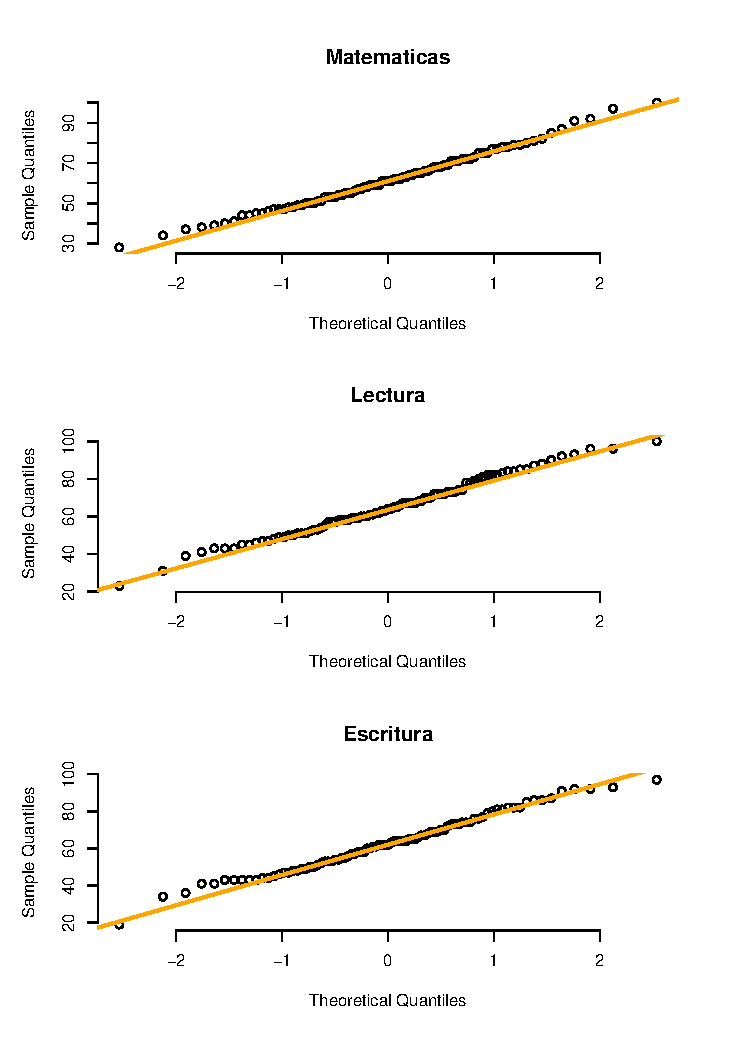
\includegraphics[scale = 0.4]{Output/Plots/qqA.eps}
            \vspace*{-6mm}
            \caption{QQplot Materias Grupo A}
            \label{fig:minipage1}
        \end{minipage}
        \hspace{0.2cm}
        \begin{minipage}[b]{0.45\linewidth}
            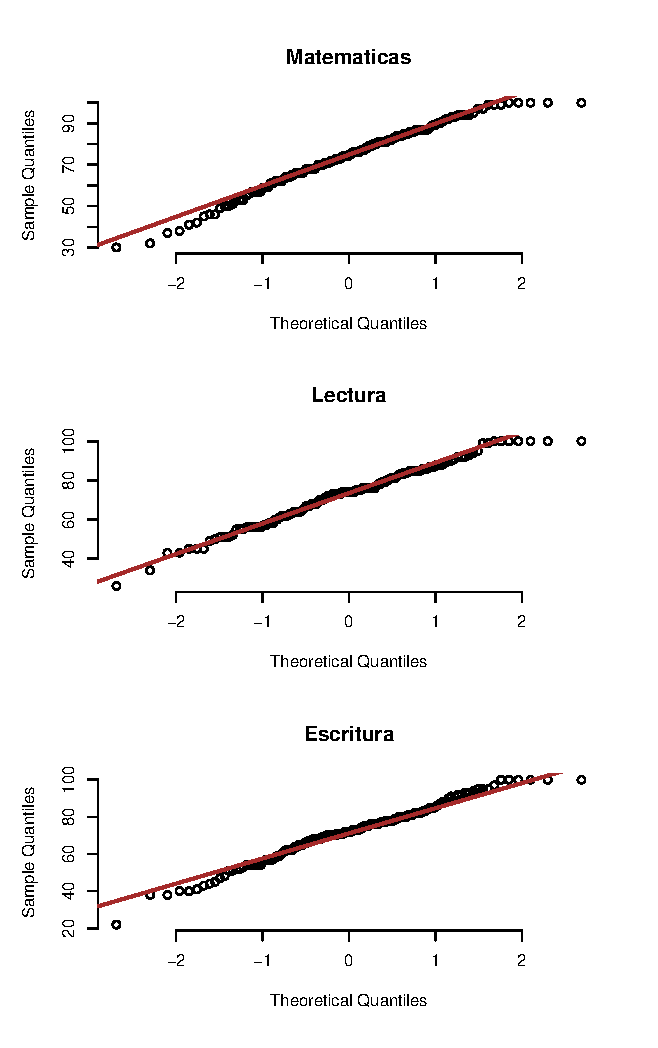
\includegraphics[scale = 0.4]{Output/Plots/qqE.eps}
            \vspace*{-6mm}
            \caption{QQplot Materias Grupo E}
            \label{fig:minipage2}
        \end{minipage}
    \end{figure}

    Es interesante ver que las notas, tanto para el grupo A como para el grupo E, parecieran
    ajustarse a una distribuci\'on normal, esto de acuerdo a las figuras 9 y 10.

    \begin{figure}[H]
        \begin{minipage}[b]{0.45\linewidth}
            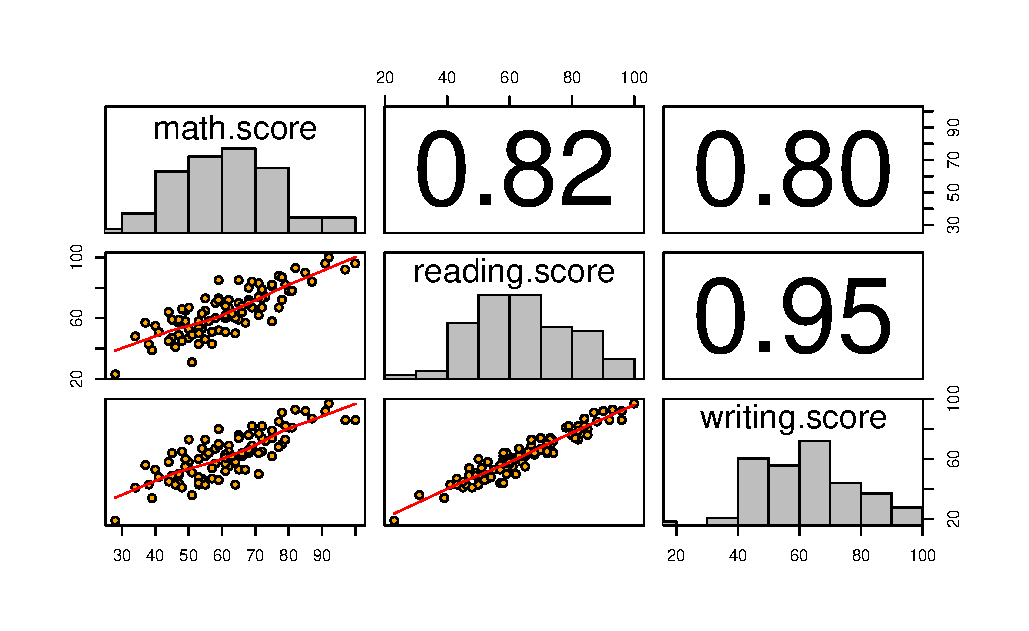
\includegraphics[width=8cm]{Output/Plots/5CorrgrupoA.eps}
            \vspace*{-8.5mm}
            \caption{Correlaci\'on entre materias. Grupo A}
            \label{fig:minipage1}
        \end{minipage}
        \hspace{0.2cm}
        \begin{minipage}[b]{0.45\linewidth}
            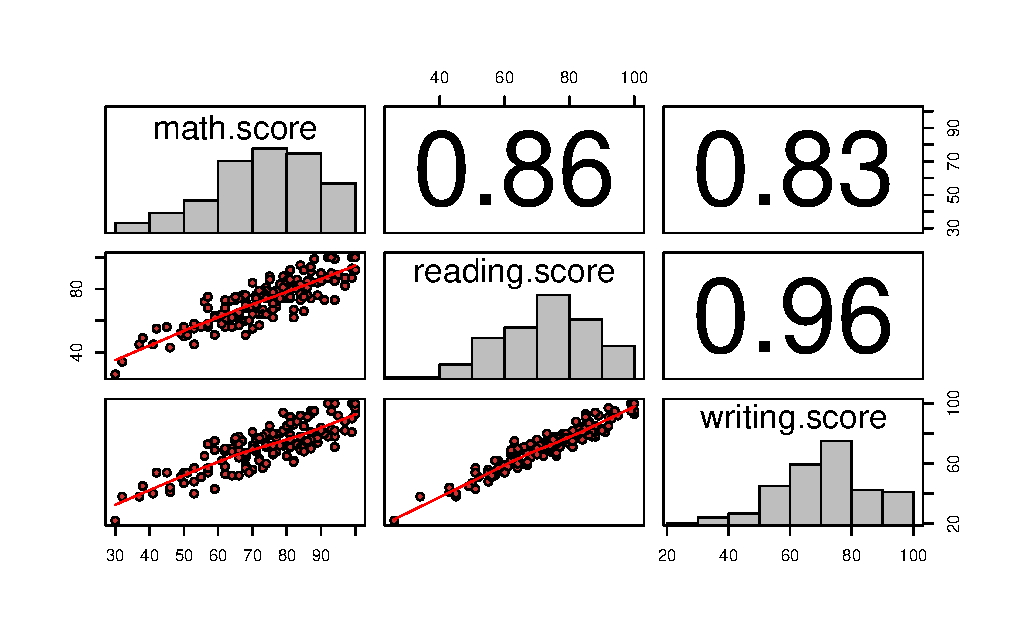
\includegraphics[width=8cm]{Output/Plots/6CorrelaciongrupoE.eps}
            \vspace*{-9mm}
            \caption{Correlaci\'on entre materias. Grupo E}
            \label{fig:minipage2}
        \end{minipage}
    \end{figure}
    \newpage
    Tanto para el grupo A como para el grupo E es evidente la calta correlaci\'on que existe entre las notas de los tres ex\'amenes,
     como nos lo confirman las figuras 11 y 12. Estas correlaciones, muy cercanas a a unidad, nos idican que el que un alumno haya salido
     bien en una prueba, con mucha probabilidad podr\'iamos afirmar que tambien obtuvo un buen resultado en la dem\'as. Lo mismo
     es cierto para el sentido contrario, un alumno con un bajo puntaje en una prueba probablemente haya salido de forma similar en la dem\'as.\\

     Esto nos lleva a la conclusi\'on que, los alumnos que lograron un bajo puntaje puede que hayan tenido tal nota debido a
     situaciones propias de sus condiciones y no por alguna dificultad intr\'inseca de la prueba.


    Una posible raz\'on para que un alumno pueda salir de manera poco satisfactoria puede ser la preparaci\'on. As\'i que analizaremos
    los resultados contrastando con los alumnos que recibieron o no, alg\'un curso de preparaci\'on.


    \begin{figure}[H]
        \begin{minipage}[b]{0.45\linewidth}
            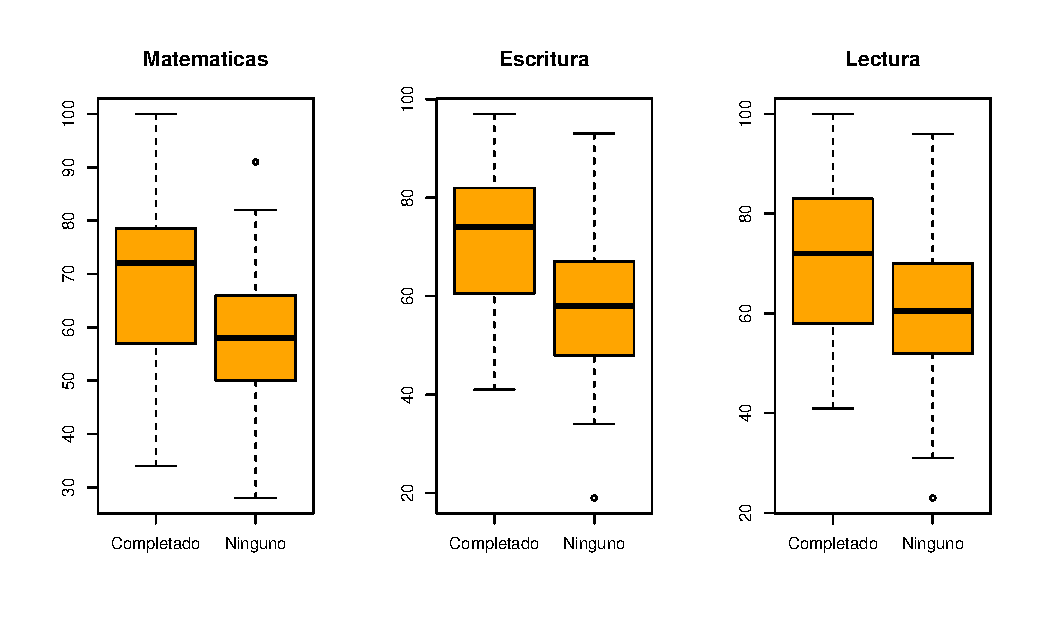
\includegraphics[width=8cm,height = 5cm]{Output/Plots/7DesempenogrupoACurso.eps}
            \vspace*{-8.5mm}
            \caption{Comparacion resultados A por curso}
            \label{fig:minipage1}
        \end{minipage}
        \hspace{0.2cm}
        \begin{minipage}[b]{0.45\linewidth}
            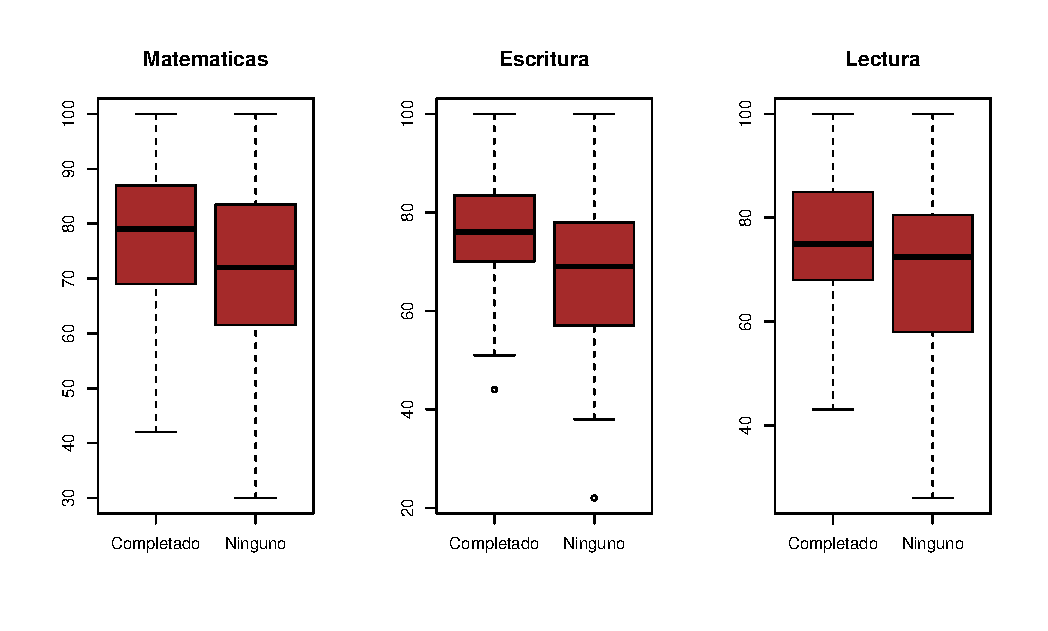
\includegraphics[width=8cm,height = 5cm]{Output/Plots/8DesempenogrupoECurso.eps}
            \vspace*{-9mm}
            \caption{Comparacion resultados E por curso}
            \label{fig:minipage2}
        \end{minipage}
    \end{figure}


    \begin{figure}[ht]
        \begin{minipage}[b]{0.45\linewidth}
            \includegraphics[width=8cm]{Output/Plots/figura9.eps}
            \vspace*{-15mm}
            \caption{Proporci\'on curso. Grupo A}
            \label{fig:minipage1}
        \end{minipage}
        \hspace{0.2cm}
        \begin{minipage}[b]{0.45\linewidth}
            \includegraphics[width=8cm]{Output/Plots/figura10.eps}
            \vspace*{-15mm}
            \caption{Proporci\'on curso. Grupo E}
            \label{fig:minipage2}
        \end{minipage}
    \end{figure}

    Como era de esperarse, los alumnos que realizaron un curso de nivelaci\'on tuvieron mejores puntajes,
    esto para todas las materias, como puede verse en la figuras 13 y 14, en promedio los estudiantes que completaron
    un curso de preparaci\'on lograron puntajes mayores que los que no.

    Comparando el n\'umero de alumnos, dentro del grupo E 60 estudiantes, de los 140, participaron en un curso de nivelaci\'on.
    Mientras que los alumnos del grupo A, s\'olo 30 de los 89 estudiantes participaron.

    Esto puede dar un indicio de el por qu\'e el grupo A obtuvo notas mas bajas que los dem\'as.


\begin{figure}[H]
        \begin{minipage}[b]{0.45\linewidth}
            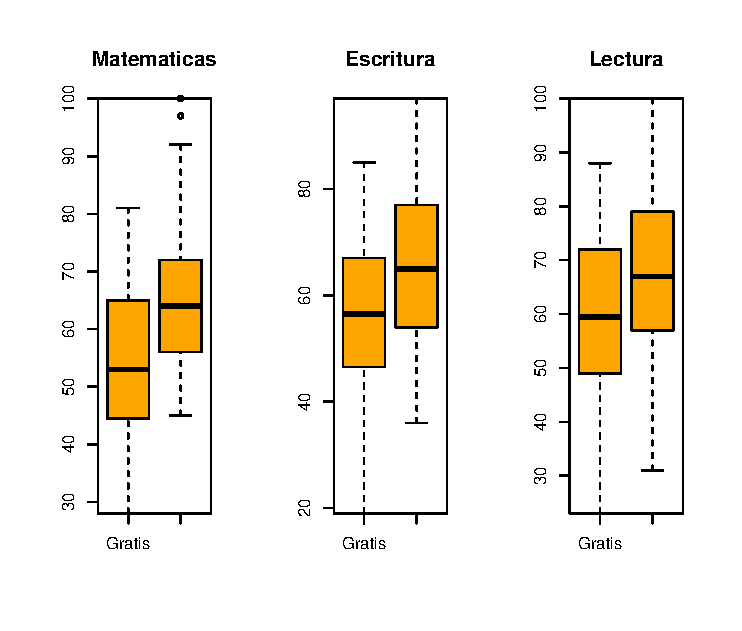
\includegraphics[width=8cm,height = 5cm]{Output/Plots/figura11.eps}
            \vspace*{-8.5mm}
            \caption{Comparacion resultados A por alimentaci\'on}
            \label{fig:minipage1}
        \end{minipage}
        \hspace{0.2cm}
        \begin{minipage}[b]{0.45\linewidth}
            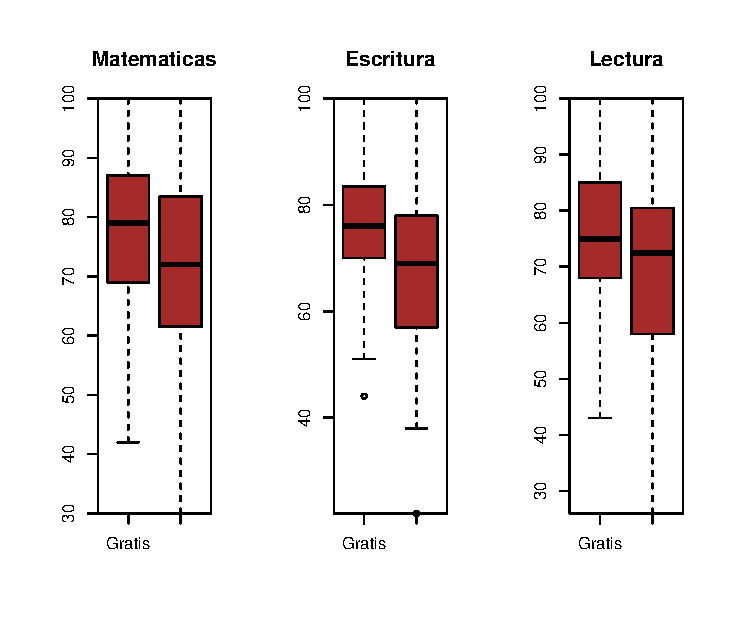
\includegraphics[width=8cm,height = 5cm]{Output/Plots/figura12.eps}
            \vspace*{-9mm}
            \caption{Comparacion resultados E por alimentaci\'on}
            \label{fig:minipage2}
        \end{minipage}
    \end{figure}

    
    \begin{figure}[H]
        \begin{minipage}[b]{0.45\linewidth}
            \includegraphics[width=8cm,height = 9cm]{Output/Plots/figura13.eps}
            \vspace*{-15mm}
            \caption{Proporci\'on almuerzo. Grupo A}
            \label{fig:minipage1}
        \end{minipage}
        \hspace{0.2cm}
        \begin{minipage}[b]{0.45\linewidth}
            \includegraphics[width=8cm,height = 9cm]{Output/Plots/figura14.eps}
            \vspace*{-15mm}
            \caption{Proporci\'on almuerzo. Grupo E}
            \label{fig:minipage2}
        \end{minipage}
    \end{figure}

    Realizando un an\'alisis de los alumnos en cuanto a su alimentaci\'on obtenemos resultados un poco diferentes.
    La diferencia entre los alumnos del grupo A y del grupo E que gozaron de un almuerzo standard es mucho menor
    que la diferencia entre los que no comieron. Al parecer los alumnos del grupo A que llegaron a tener un almuerzo
    completo lograron puntajes mucho m\'as altos que los que no. 
    En total en el grupo A s\'olo 35, de 89 alumnos, pudieron acceder al almuerzo completo
    mientras que para la secci\'on E fueron 98 alumnos, de 140. 
    

    \begin{figure}[H]
        \noindent\makebox[\textwidth]{
        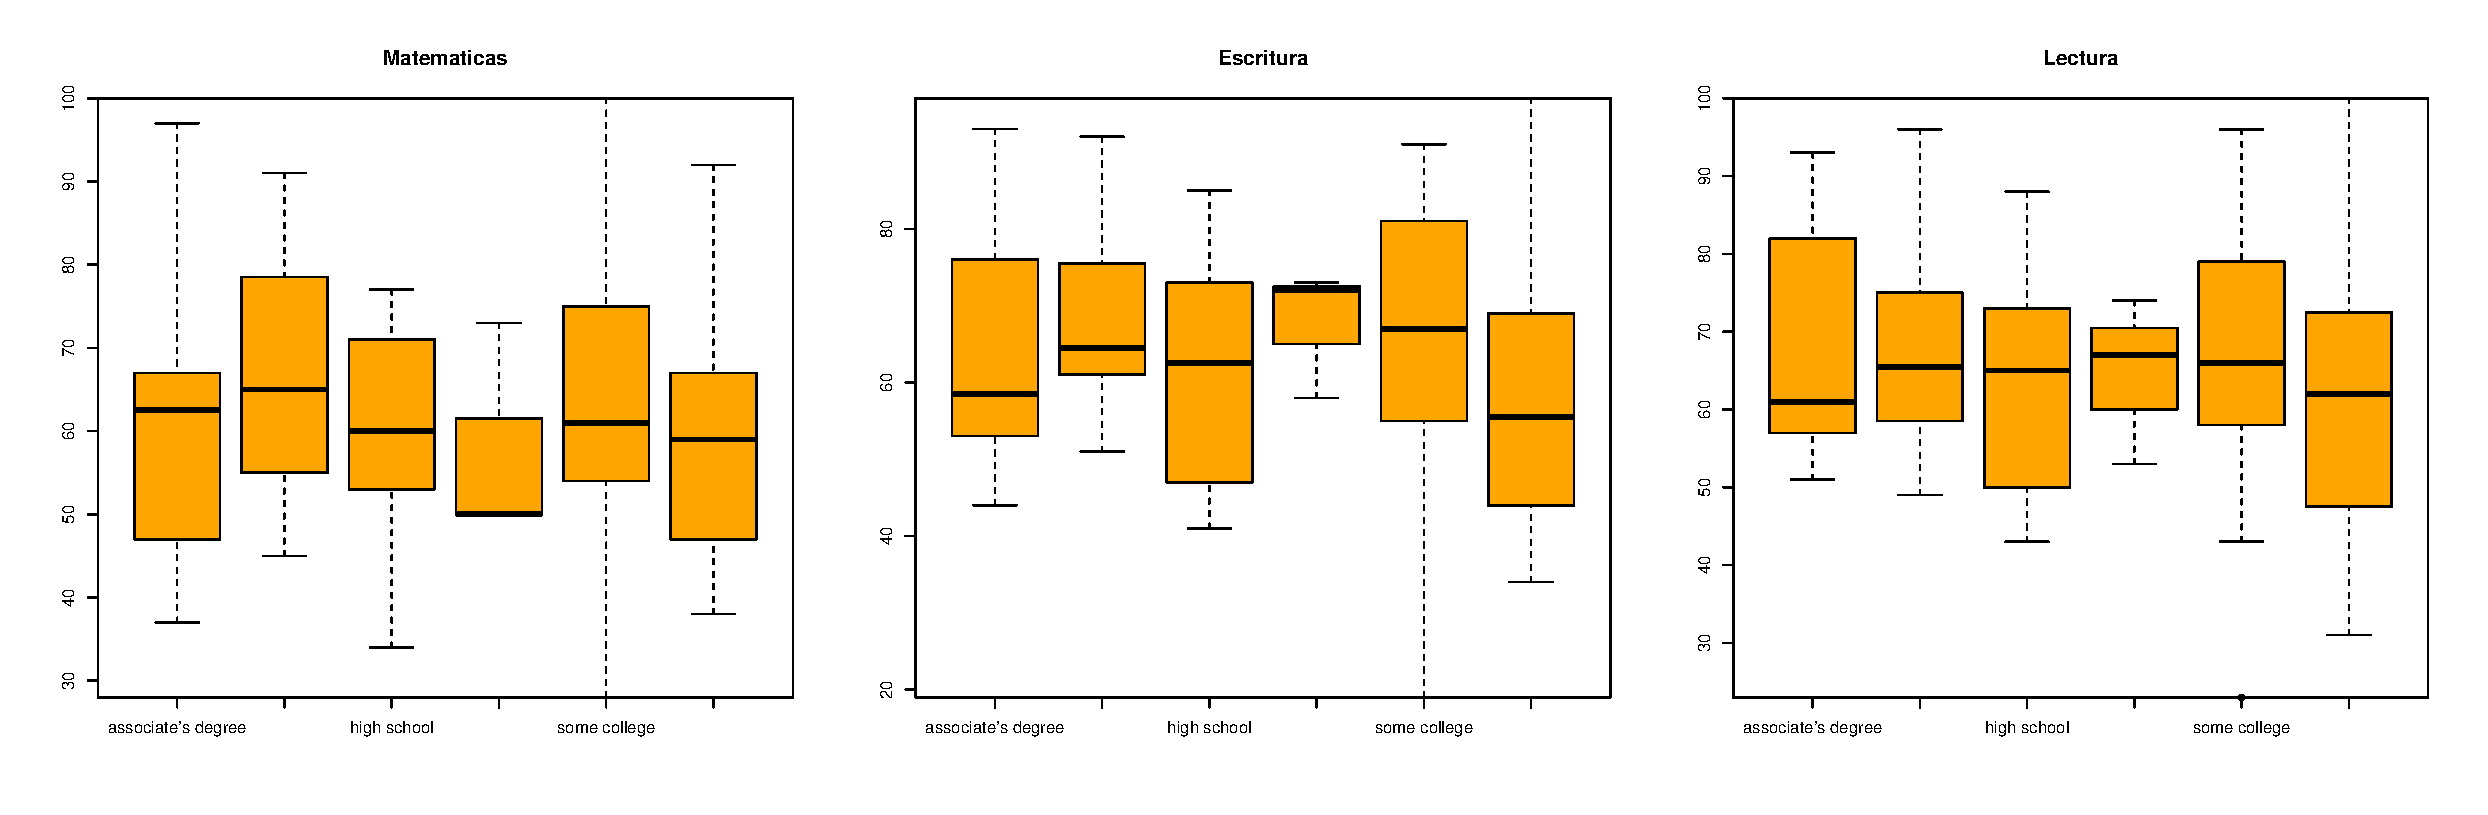
\includegraphics[width = 17 cm, height = 6cm ]{Output/Plots/figure15.eps}}
        \caption{Resultados del grupo A por grado educativo de los padres}
        \label{fig:minipage1}
    \end{figure}

    \begin{figure}[H]
        \noindent\makebox[\textwidth]{
        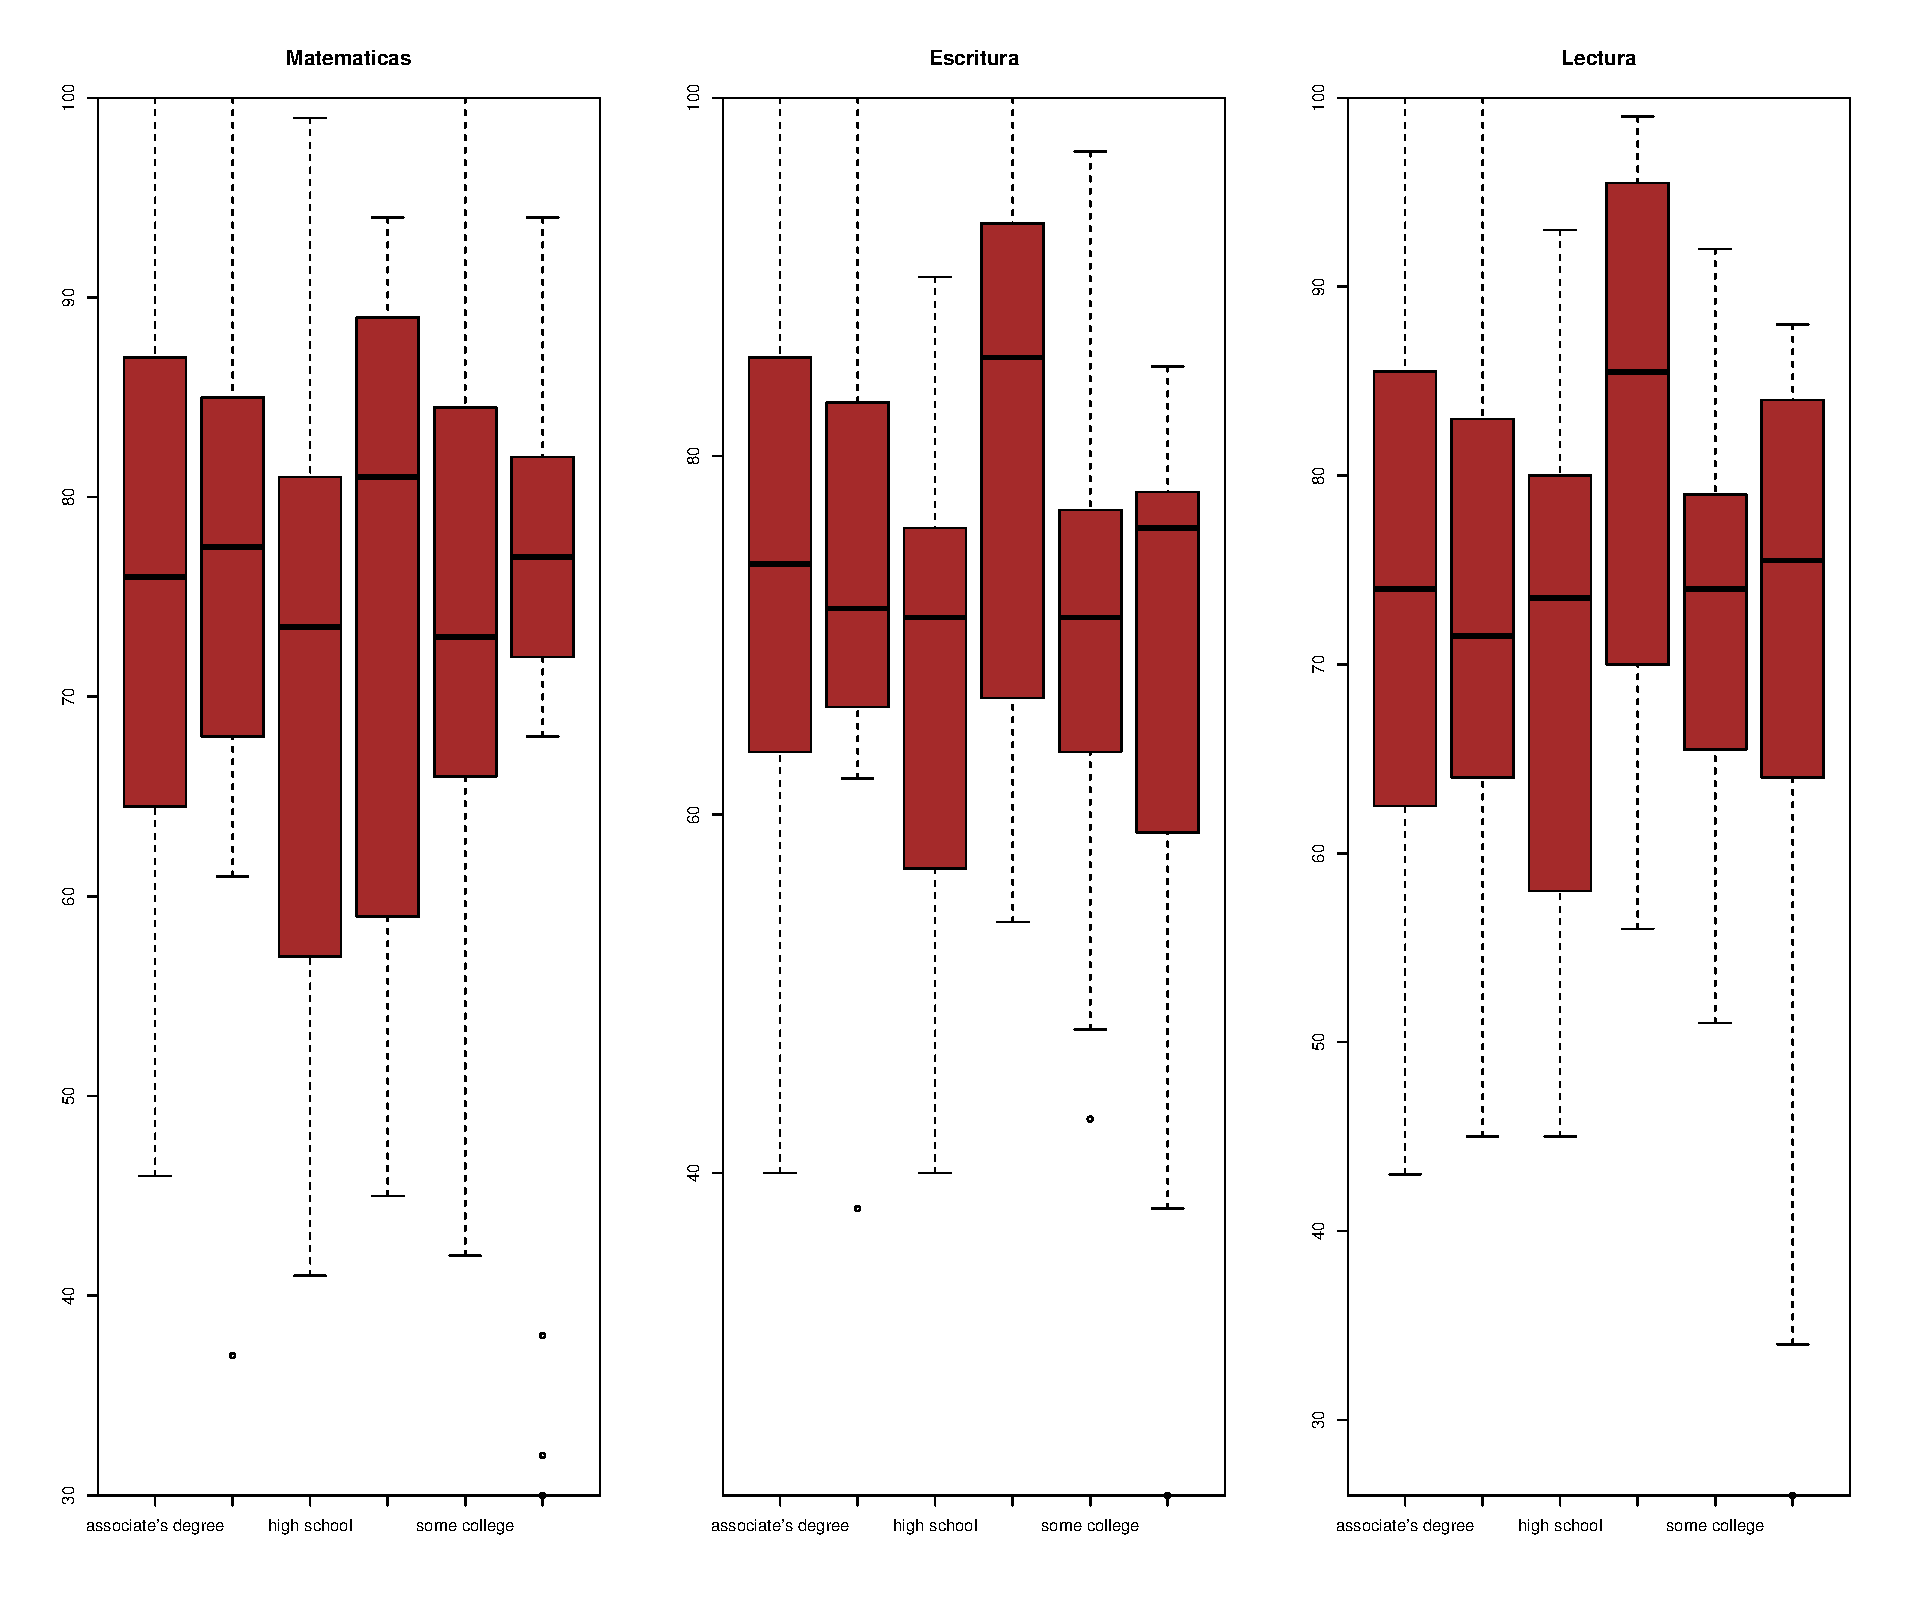
\includegraphics[width = 17 cm, height = 6cm ]{Output/Plots/figure16.eps}}
        \caption{Resultados del grupo E por grado educativo de los padres}
        \label{fig:minipage1}
    \end{figure}



    \begin{figure}[H]
        \begin{minipage}[b]{0.45\linewidth}
            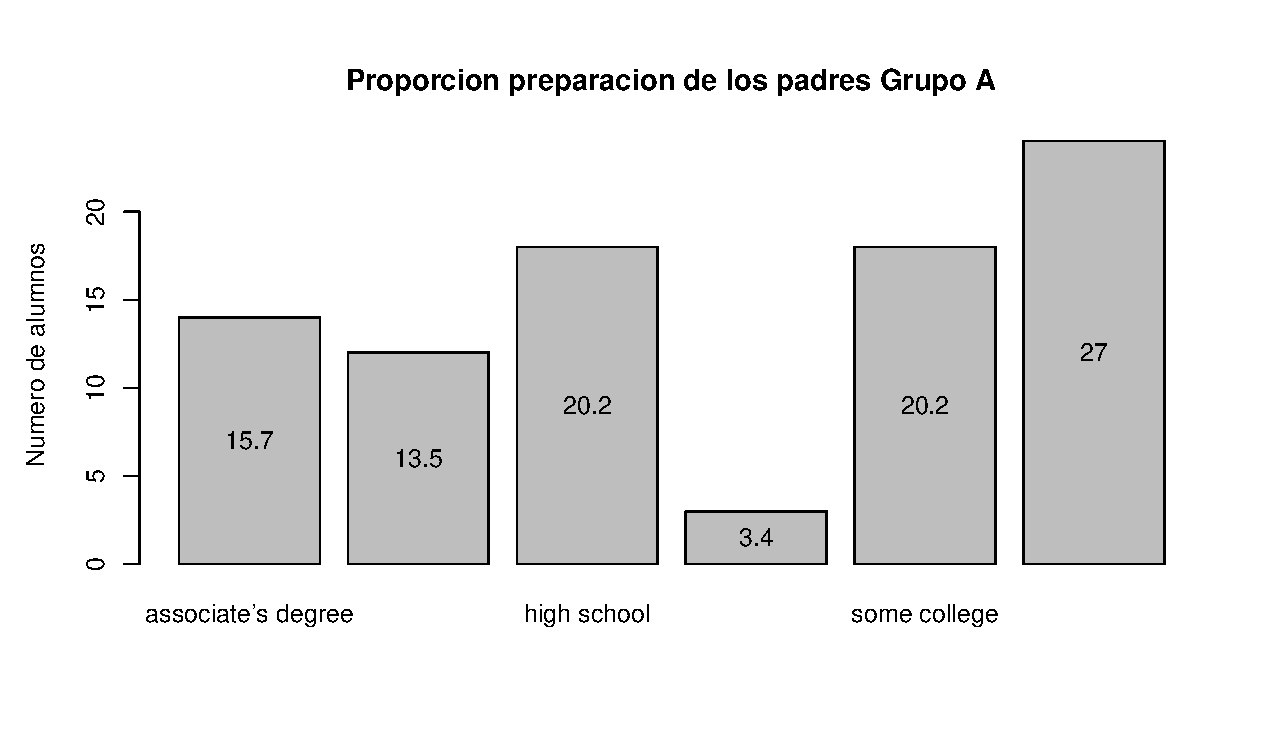
\includegraphics[width=8cm,height = 5cm]{Output/Plots/figure17.eps}
            \vspace*{-8.5mm}
            \caption{Comparacion resultados A por educaci\'on de los padres}
            \label{fig:minipage1}
        \end{minipage}
        \hspace{0.2cm}
        \begin{minipage}[b]{0.45\linewidth}
            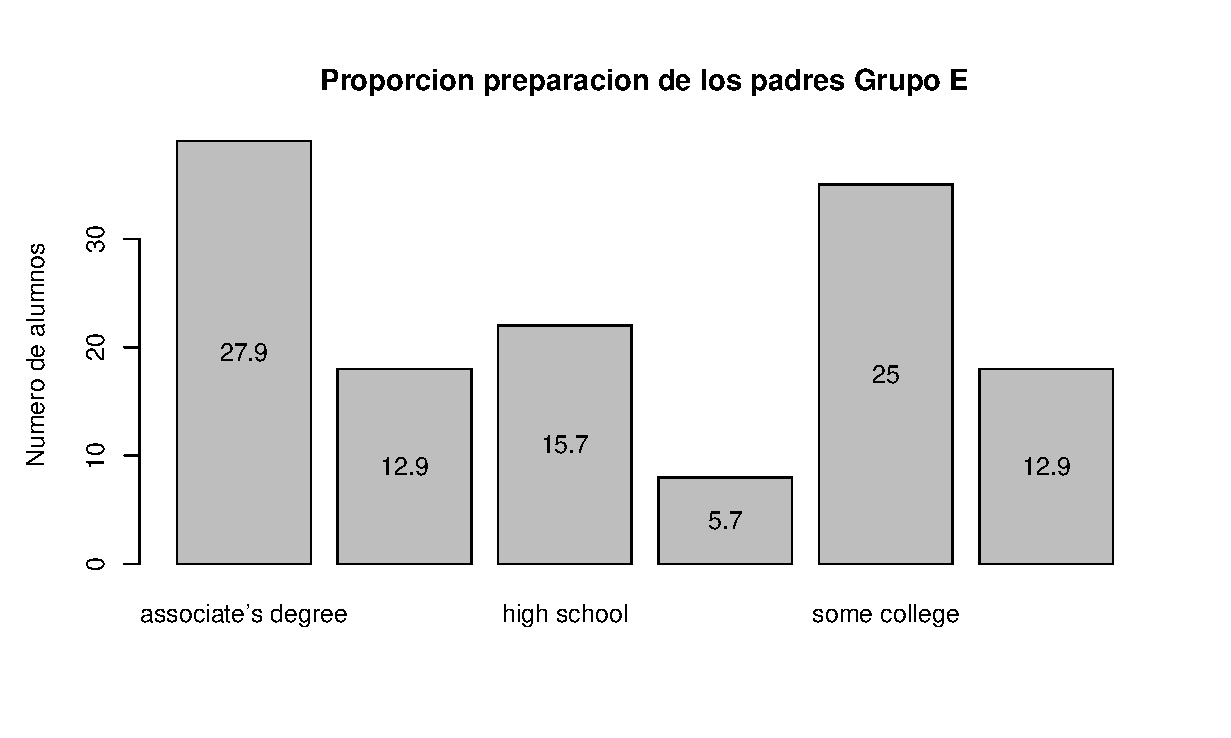
\includegraphics[width=8cm,height = 5cm]{Output/Plots/figure18.eps}
            \vspace*{-9mm}
            \caption{Comparacion resultados E por educaci\'on de los padres}
            \label{fig:minipage2}
        \end{minipage}
    \end{figure}


    Analizando ambos grupos respecto al nivel educativo de sus padres podemos ver que, en las figuras 23 y 24, no 
    hay una tendencia aparente sobre un subgrupo a otro. Que un estudiante provenga de un hogar con padres
    con alto nivel educativo no tiene aparente influencia en su desempe\~no. De igual forma, revisando la proporci\'on,
    podemos ver que no hay un grupo predominante, a excepci\'on de los alumnos de padres con master que es mucho menor
    que los dem\'as, sin embargo su desempe\~no no parece ser muy alejado de los dem\'as estudiantes.

    Un \'ultimo par\'ametro que podemos analizar es, el genero, verificaremos si el genero de alg\'un estudiante

    \begin{figure}[H]
        \begin{minipage}[b]{0.45\linewidth}
            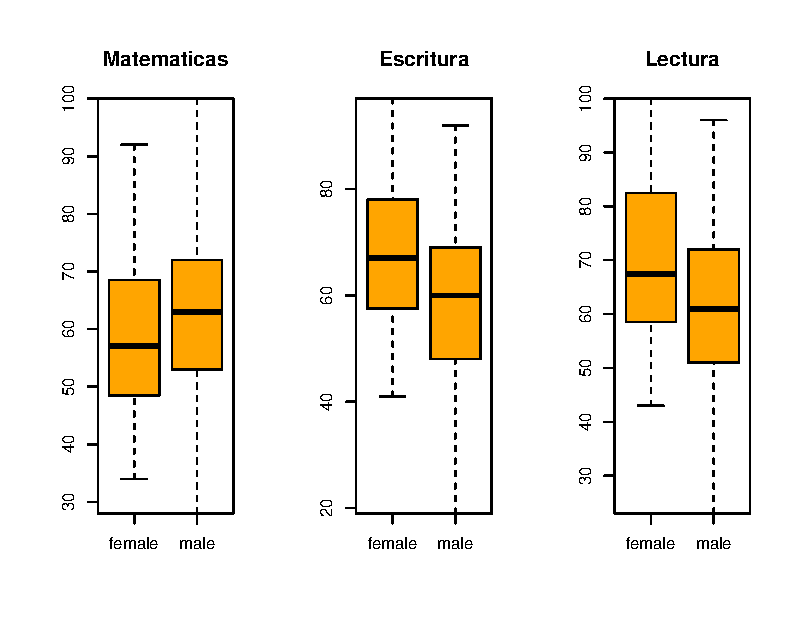
\includegraphics[width=8cm,height = 5cm]{Output/Plots/figure19.eps}
            \vspace*{-8.5mm}
            \caption{Comparacion resultados A por g\'enero}
            \label{fig:minipage1}
        \end{minipage}
        \hspace{0.2cm}
        \begin{minipage}[b]{0.45\linewidth}
            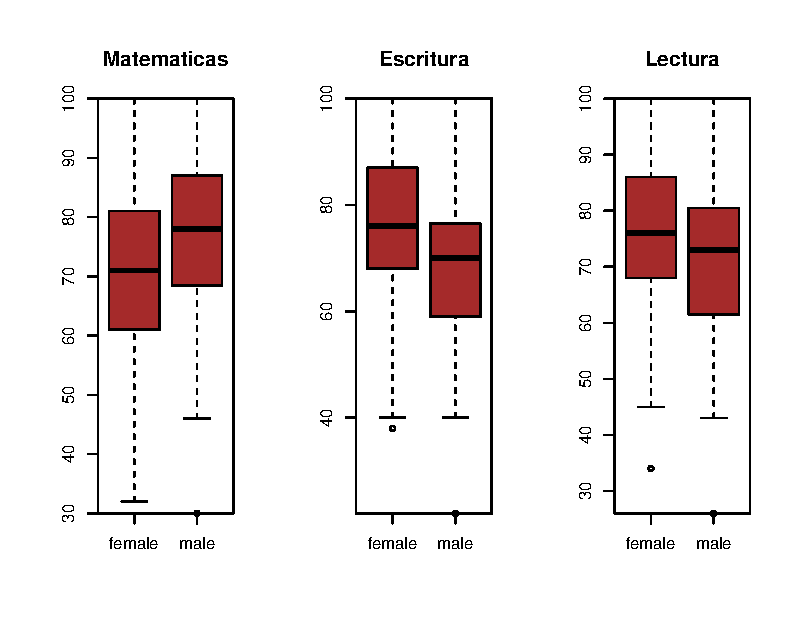
\includegraphics[width=8cm,height = 5cm]{Output/Plots/figure20.eps}
            \vspace*{-9mm}
            \caption{Comparacion resultados E por g\'enero}
            \label{fig:minipage2}
        \end{minipage}
    \end{figure}


    \begin{figure}[H]
        \begin{minipage}[b]{0.45\linewidth}
            \includegraphics[scale = 0.8]{Output/Plots/figure21.eps}
            \vspace*{-8.5mm}
            \caption{Representaci\'on de g\'enero grupo A}
            \label{fig:minipage1}
        \end{minipage}
        \hspace{0.2cm}
        \begin{minipage}[b]{0.45\linewidth}
            \includegraphics[scale = 0.8]{Output/Plots/figure22.eps}
            \vspace*{-9mm}
            \caption{Representaci\'on de g\'enero grupo E}
            \label{fig:minipage2}
        \end{minipage}
    \end{figure}

    De las figuras 25 y 26 podemos ver que los alumnos de g\'enero masculino tienden a salier mucho mejor
    en matem\'aticas mientras que las alumnas de g\'enero femenino, en su mayor\'ia, salieron mejor
    en las materias de escritura y lectura.

    Sin embargo podemos notar que, en el grupo E, el porcentaje de estudiantes de g\'enero femenino 
    es mucho mayor que en el grupo A.\\

    Resumiendo todo lo anterior podemos aseverar que los alumnos del grupo A tuvieron un desempe\~no
    mucho menos satisfactorio que los dem\'as grupos, en particular el E, debido a tener serias desventajas
    tales como falta de alimentaci\'on completa y acceso a un refuerzo educativo adem\'as de 
    tener poca representaci\'on del g\'enero femenino. 
    
    \begin{figure}[H]
            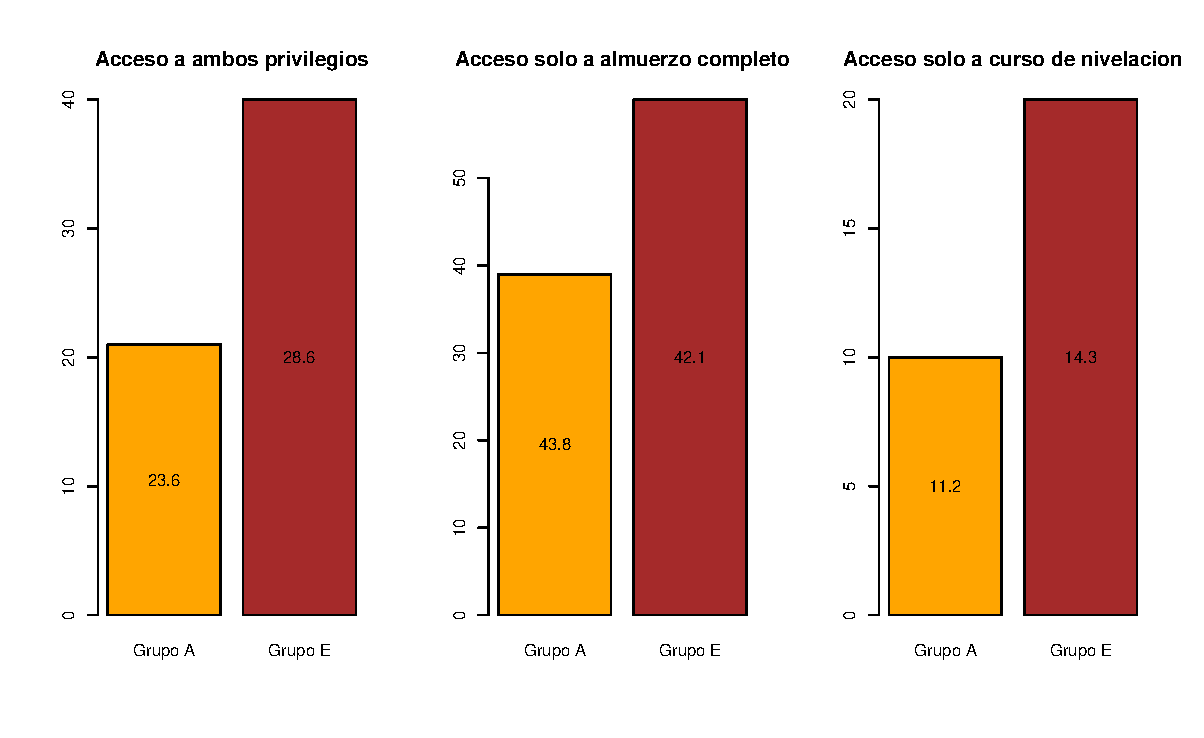
\includegraphics[scale = 0.7]{Output/Plots/privilegios.eps}
            \vspace*{-6mm}
            \caption{Comparaci\'on de acceso a los distintos privilegios}
    \end{figure}

    Como podemos ver en la figura 29, el acceso a tanto a ambos privilegios, como a uno s\'olo en particular,
    fue mucho m\'as alto en el grupo E que en el grupo A. En el grupo A el porcentaje de acceso a alg\'un privilegio
    es relativamente bajo.
    
    \begin{figure}[H]
        \centering
        \includegraphics[scale = 0.5]{Output/Plots/sinprivilegio.eps}
        \vspace*{-6mm}
        \caption{Comparaci\'on entre el grupo A y E sin privilegios}
    \end{figure}

    Como es evidene, en la figura 30 podemos confirmar, el procentaje de alumnos del grupo A que no 
    tuvieron acceso a ning\'un privilegio es mayor que los del grupo E.

    En conclusi\'on, los alumnos del grupo \'etnico A no tuvieron un desempe\~no satisfactorio
    respecto a las dem\'as secciones debido a que en muchos casos, los alumnos de este grupo
    no tuvieron acceso a ciertos privilegios que pudieran 
\end{document}